\documentclass[11pt]{article}
\usepackage{setspace}
\usepackage{cite}
\usepackage{graphicx}
\usepackage{url}
\usepackage{listings}
\usepackage{amsmath}

\newcommand{\Rpackage}[1]{\emph{#1}}
\newcommand{\tigre}[0]{\Rpackage{tigre}}

\lstset{language=R,basicstyle=\footnotesize}

\title{Mining regulatory network connections by ranking transcription
  factor target genes using time series expression data}
\author{Antti Honkela, Magnus Rattray, and Neil D.\ Lawrence}

\begin{document}
\maketitle

\begin{abstract}
Reverse engineering the gene regulatory network is challenging because
the amount of available data is very limited compared to the
complexity of the underlying network.  We present a technique
addressing this problem through focussing on a more limited problem:
inferring direct targets of a transcription factor from short
expression time series.  The method is based on combining Gaussian
process priors and ordinary differential equation models allowing
inference on limited potentially unevenly sampled data.  The method is
implemented as an R/Bioconductor package and it is demonstrated by
ranking candidate targets of the p53 tumour suppressor.
\end{abstract}

\onehalfspacing

\section{Introduction}

Understanding the function and regulation of all human genes is one of
the most important challenges that needs to be solved to fully ripe
the benefits of the Human Genome Project and the genomic era.

There are several regulatory mechanisms affecting protein expression.
We will focus on transcriptional regulation, which is mediated by
transcription factors (TFs).  They are proteins that bind the DNA to
activate or repress the transcription of their target genes.  The
relationships between TFs and their target genes can be represented as
a graph which is called the gene regulatory network.  In reality, this
network is context-sensitive with many connections being, for
instance, tissue specific.

Inferring the gene regulatory network from data is a very challenging
problem.  Even with the high-throughput measurement techniques
providing data on a genome-wide scale, the amount of data is tiny
compared to the potential complexity of the regulatory network.
Taking a conservative estimate of 1500 human TFs~\cite{Vaquerizas2009}
regulating some 22500 genes~\cite{Pertea2010a} yields an astronomical
number of more than $10^{450}$ potential networks.  Even with a more
realistic assumption of at most 5 regulating TFs for each gene there
are more than $10^{18}$ potential networks, or from another
perspective more than $6.3 \cdot 10^{13}$ potential sets of regulators
for each gene.  Assuming the regulatory network can be captured by a
differential equation model with as many parameters, twice as many
experiments would be needed to identify all the
parameters~\cite{Sontag2002}.  If a simplified model of regulation
with fewer parameters (such as a linear differential equation) can be
assumed, the number of experiments will drop
accordingly~\cite{Stark2003}, but naturally such a model cannot
capture all possible modes of combinatorial regulation.

The difficulty of general network inference even for simpler organisms
was recently demonstrated by the DREAM5 Network Inference
challenge\footnote{See
  \url{http://wiki.c2b2.columbia.edu/dream/results/DREAM5/?c=4_1}},
where one of the tasks was to infer the regulatory network for yeast
using practically all available expression data.  As a result, the
best-performing team in this subtask achieved an area under the ROC
curve of 0.539, which is only marginally better than the result 0.5
corresponding to random guessing.

\subsection{Probabilistic dynamical models or gene regulation}

To avoid these difficulties, we will focus on a specific task of
identifying the targets of a TF in a time series experiment where the
TF activity is changing~\cite{Gao2008,Honkela2010PNAS}.  The method
works based on expression data alone.  The TF activity can be
estimated using information from known target genes or using the TF
mRNA, if the TF is assumed to be primarily under transcriptional
control.  Given an estimate of TF activity and a model of
transcription based on this activity, we can rank candidate targets
based on how well they fit the model of regulation by this TF.

As our model of gene transcription regulated by a TF and optionally
TF protein translation we use the following linear ordinary
differential equations (ODEs):
\begin{align}
  \frac{\mathrm{d}p(t)}{\mathrm{d}t} & = f(t) - \delta
  p(t) \ , \label{eq:translation_ode} \\
  \frac{\mathrm{d}m_j(t)}{\mathrm{d}t} & = B_j+S_j p(t)-D_j m_j(t) \ , \label{eq:transcription_ode}
\end{align}
where $p(t)$ is the TF protein at time $t$, $m_j(t)$ is the $j$th
target mRNA concentration and $f(t)$ is the TF mRNA. The parameters
$B_j$, $S_j$ and $D_j$ are the baseline transcription rate,
sensitivity and decay rate respectively for the mRNA of the $j$th
target as described in \cite{Barenco2006a}.  The parameter
$\delta$ is the decay rate of the TF protein~\cite{Honkela2010PNAS}.

In order to infer the protein activity $p(t)$, we need a prior for it.
As the functions $f(t), p(t)$ and $m_j(t)$ are deterministically
linked by the ODEs, this can be accomplished by placing a Gaussian
process prior on $f(t)$ \footnote{If the TF protein is under
  significant post-translational regulation,
  Eq.~(\ref{eq:translation_ode}) may be omitted and the prior placed
  directly on $p(t)$.  In this case multiple known targets are needed
  to reliably infer $p(t)$.}.
This leads to a joint Gaussian process over the three continuous-time
functions $f(t),p(t)$ and $m_j(t)$.  Data are observations of the
expression levels at arbitrary specific times (not necessarily evenly
spaced) and we assume a Gaussian noise model: $\hat{m}_j(t_i) \sim
N(m_j(t_i),\sigma_{i,m_j}^2)$ and $\hat{f}(t_i) \sim
N(f(t_i),\sigma_{i,f}^2)$ with known (derived from \emph{puma}, see
below) or estimated gene-specific noise variance parameters. The
parameters of the model as well as other parameters of the Gaussian
process covariance are optimised by maximising the marginal
likelihood.

\subsection{Related approaches}

Other approaches for ranking TF targets using similar data include the
rHVDM package~\cite{Barenco2009} which implements a non-probabilistic
variant of the same transcription ODE model~\cite{Barenco2006a}.
rHVDM does not support using the TF mRNA observations to infer TF
activity.  Another alternative that defines the model based only on
TF expression data without a possibility of using information from the
targets to infer TF activity is TSNI~\cite{Gatta2008}.

In general, the main difficulty in linking putative target genes with
their regulators using expression data are the different degradation
rates of mRNA molecules of different genes.  If the degradation rates
are available and can be compensated for, estimation of the regulator
activation profiles is greatly simplified~\cite{Barenco2009a}.  Our
method can easily use such information as well.

\section{Materials}

The presented target ranking approach is implemented in the \tigre{}
package which is available in Bioconductor~\cite{Gentleman2004} for R
(since Bioconductor 2.6 for R-2.11).  \tigre{} can make effective use
of error estimates for expression levels provided by preprocessing
methods.  For Affymetrix arrays these are most easily available from
the Bioconductor package \Rpackage{puma}~\cite{Pearson2009}, for
Illumina arrays the corresponding information is available from
Bioconductor package \Rpackage{lumi}~\cite{Du2008}.

\section{Methods}

\subsection{Data collection and experimental design}

The primary data used by the model are expression time series.  They
can be measured using any quantitative technique such as mRNA
sequencing (RNA-seq) or microarrays.

The application of our ranking method requires time series data.  Due
to financial constraints, most biological time series are very short,
which poses problems for data modelling.  We have applied the ranking
to data sets with as few as 6--7 time
points~\cite{Honkela2010MLSP,Honkela2010PNAS}, although longer time
series ($> 10$ time points) are significantly more informative.

Given a fixed experimental budget, it seems in general preferable to
have more experimental perturbations and more finely sampled time
series rather than more replicates of the same measurements, except
possibly for some single key time points.  The models can use
continuity in the time series to compensate for the noise that is
usually detected using the replicates.

\subsection{Preprocessing}

The expression data should be preprocessed using the best tools for
that particular platform.  The \tigre{} ranking method can make use of
error or variance estimates from preprocessing.  At the time of
writing, first such tools for RNA-seq data are only becoming
available.  For microarrays, for example the
\Rpackage{puma}~\cite{Pearson2009} Bioconductor package provides such
estimates for Affymetrix GeneChips, while the
\Rpackage{lumi}~\cite{Du2008} package provides this for Illumina Bead
Arrays.

In order to use the data with \tigre{}, it must be imported using the
function \texttt{processData} that normalises the output from
\Rpackage{puma} and \Rpackage{lumi}, or \texttt{processRawData} that
handles plain expression data matrices.  These functions require
information about the experimental setup of the data, including
observation times of different samples and which replicate time series
they belong to.  An example of the preprocessing using the p53
activation data from~\cite{Barenco2006a} is presented below.  More
details are available in the vignettes and other documentation of the
respective packages.

\begin{lstlisting}[frame=single]
library(ArrayExpress)

## Get data from ArrayExpress
p53.affybatch <- ArrayExpress('E-MEXP-549')
## Sort the arrays in a sensible order
mynames <- rownames(pData(p53.affybatch))
I <- order(strtrim(mynames, 5),
           pData(p53.affybatch)['Factor.Value..time.'])
p53.affybatch <- p53.affybatch[,I]

## Run mmgMOS preprocessing
library(puma)
p53.exprReslt <- mmgmos(p53.affybatch)

## Run tigre data normalisation
exps <- rep(1:3, each=7)     # replicates: 1...12...23...3
p53.timeseries <- processData(p53.exprReslt, experiments=exps)
\end{lstlisting}

\subsection{Ranking}

Ranking candidate targets of a TF requires inferring the TF activity
profile.  This can be done using TF mRNA expression levels if the TF
can be assumed to be under transcriptional control, or using
expression data of known targets, or combining both.  Both of these
cases are handled by the \tigre{} function \texttt{GPRankTargets}.

If known targets are available, the function first fits a model using
these known targets to infer the TF activity.  All other genes are
then screened by fitting additional models by adding then to the
target set one at a time.  If there are no known targets, all genes
are screened by simply fitting them one at a time.
In our p53 example this is achieved using the below code.

\begin{lstlisting}[frame=single]
## Known target probes from Barenco et al. (2006)
## These are the most informative probes for genes
## 'DDB2', 'CDKN1A', 'PA26', 'BIK', 'TNFRSF10B'
knownprobes <- c('203409_at', '202284_s_at', '218346_s_at',
                 '205780_at', '209295_at')

## Run the ranking.  This may take several hours to run.
## Results are saved to file 'p53ranking.RData'.
scores <- GPRankTargets(p53.timeseries, knownTargets=knownprobes,
                        scoreSaveFile='p53ranking.RData')

## Sort the list according to likelihood
scores <- sort(scores, descending=TRUE)

## Find 10 top-ranking probes
genes(scores)[1:10]

## Find the corresponding gene symbols
library(annotate)
mget(unlist(genes(s)[1:10]),
     getAnnMap('SYMBOL', annotation(p53.timeseries)))
\end{lstlisting}

\subsection{Visualisation and analysis}

The most effective way to explore the ranking results is by looking at
visualisations of the models.  Given the over 10000 models produced in
the above analysis, this can be a daunting task without proper tools.
A very useful tool for browsing the models is the \emph{tigreBrowser}
tool\footnote{tigreBrowser is available for download at
  \url{http://users.ics.tkk.fi/ahonkela/tigre/}.}  The scores and the
corresponding model visualisations can be exported for
\emph{tigreBrowser} as below.

\begin{lstlisting}[frame=single]
## Export the scores and model visualisations to tigreBrowser
export.scores(scores, datasetName='Barenco2006',
              experimentSet='GPSIM 5 known',
              database='p53_results.sqlite',
              preprocData=p53.timeseries)
\end{lstlisting}

The results can then be viewed most easily by running the
\texttt{tigreServer.py} script and pointing it to the saved
\texttt{p53\_results.sqlite} file.

As there is no suitable genome-wide validation data available, we used
a sequence-based method of validation.  To do this, we looked for
strong occurrences of the known p53 binding motif in the promoters of
highly ranked targets.  This was done by using the \texttt{p53scan}
tool of Smeenk et al.~\cite{Smeenk2008} on the sequences of 5000 bp
upstream of annotated transcription starts of RefSeq genes with
annotated 5' UTRs downloaded from hg19 assembly in the UCSC Genome
Browser~\cite{Fujita2011}.  Figure~\ref{fig:p53_validation} shows the
enrichment of the strongest $10 \%$ of the binding motif instances
identified by \texttt{p53scan} as ranked by the score on the promoters
of highly ranked genes.  While these high scoring motif instances are
the most likely true binding sites, some of them may still be
non-functional.  On the other hand, it is likely that many other genes
are regulated through a weaker site on the promoter or a more distant
site which cannot be detected without additional information.

\begin{figure}[htb]
  \centering
  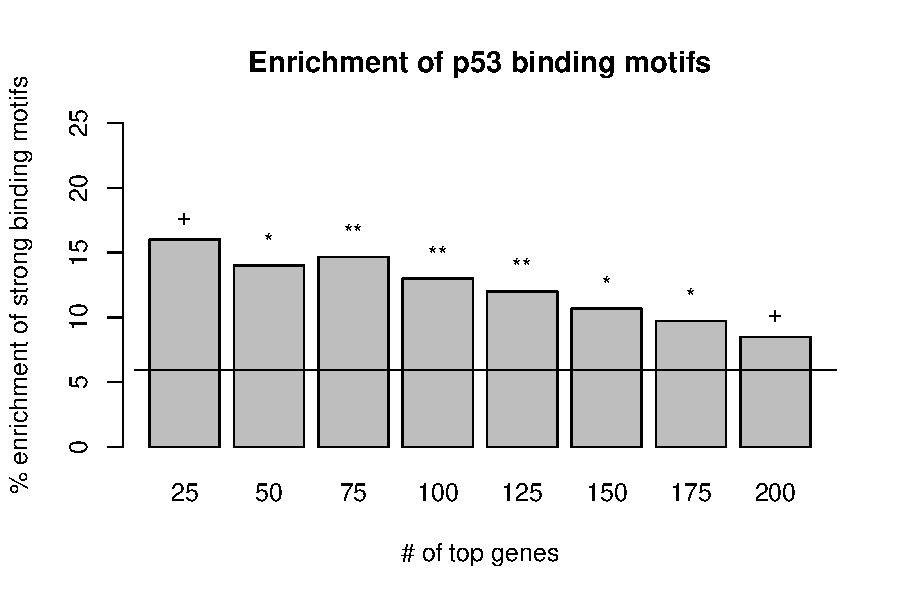
\includegraphics[width=.7\textwidth]{p53_validation}
  \caption{Enrichment of strong p53 binding motifs in the promoters of
    selected number of top predicted targets.  $p$-values of the
    enrichments are denoted by `***': $p < 0.001$, `**': $p < 0.01$,
    `*': $p < 0.05$, '+': $p < 0.1$ (tail probability in
    hypergeometric distribution).}
  \label{fig:p53_validation}
\end{figure}

\section{Notes}

One critical question in applying \tigre{} is whether to use the TF
mRNA data.  The extra information can potentially greatly help in
identifying the TF activity profile and hence making better
predictions of new targets, but it can also lead to incorrect
predictions if it turns out incorrect.  Based on our experience, the
critical question is whether some outside influence, such as a
external signal, is the rate-limiting factor in the production of the
active TF.  Simple post-translational modifications such as
dimerisation to not appear to significantly hinder the use of TF mRNA
data, as witnessed by the results in~\cite{Honkela2010PNAS} for
Drosophila TFs Mef2 and Twi which are known to function as dimers.

\bibliography{mimb_book}
\bibliographystyle{unsrt}

\end{document}
